
\chapter{Creation of GCS wireless network} \label{app:network}

The wireless network to which the OCAS will be connected for communication with the GCS shall meet two major requirements:
\begin{enumerate}
	\item The network shall allow the wireless communication between the OCAS and the GCS via SSH protocol
	\item The network should provide the OCAS with an internet connection (to allow for an easier Python scripts updating, programming, and debugging and the download of logs for analysis at the GCS via \texttt{git})
\end{enumerate}

Additionally, since the GCS consists of a Windows laptop, the tools to be used shall be compatible with the Windows 10 Operating System.

The simplest network architecture that allows for peer-to-peer communication of computers is the ad-hoc network.
Furthermore, Windows 10 Professional provides all the tools required to create such a network, which will additionally share its main Internet connection with their peers when available.

The steps to be followed on the GCS for a successful connection of the OCAS to the Windows machine are:
\begin{enumerate}
	\item Open a Command Prompt window as Administrator (network commands cannot be run by regular users for safety reasons)

	\item Create a new ad-hoc network by running the command: 

		\hspace{0.05\textwidth}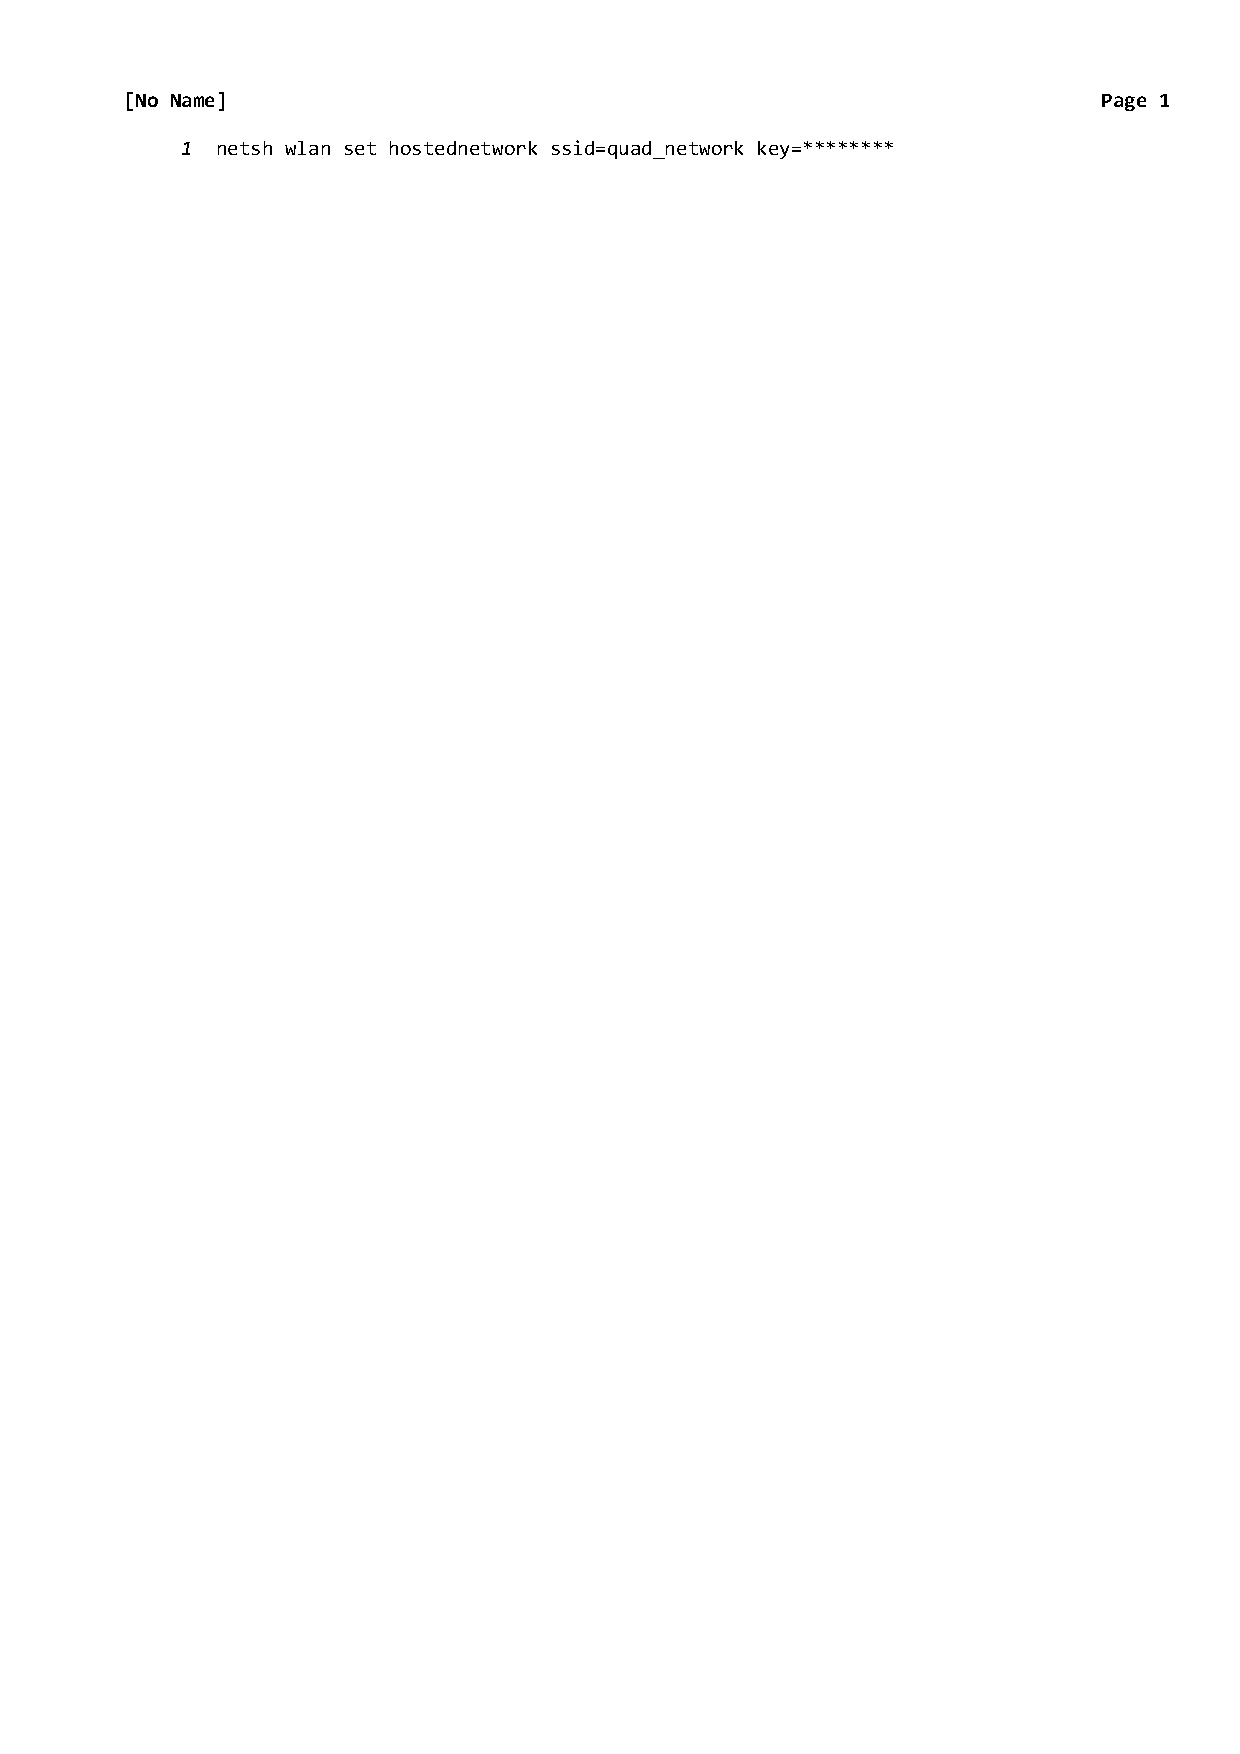
\includegraphics[width=0.95\textwidth,clip,trim={3.5cm 27cm 0 2.3cm}]{./files/setnetwork.pdf}

	\item Start the newly created network, making it available for other devices to connect:

		\hspace{0.05\textwidth}
\includegraphics[width=0.95\textwidth,clip,trim={3.5cm 27cm 0 2.3cm}]{./files/startnetwork.pdf}

	\item Edit the \texttt{wpa\_suplicant.conf} file on the Raspberry Pi to include the settings from the ad-hoc network (see example in Appendix \ref{app:interfaces})

	\item If the Raspberry Pi does not automatically connect to the network, restart the wireless interface by running:

		\hspace{0.05\textwidth}
\includegraphics[width=0.95\textwidth,clip,trim={3.5cm 26.5cm 0 2.3cm}]{./files/restartif.pdf}

	\item Check that the Raspberry Pi is connected to the Windows' network by checking the MAC address of connected devices:

		\hspace{0.05\textwidth}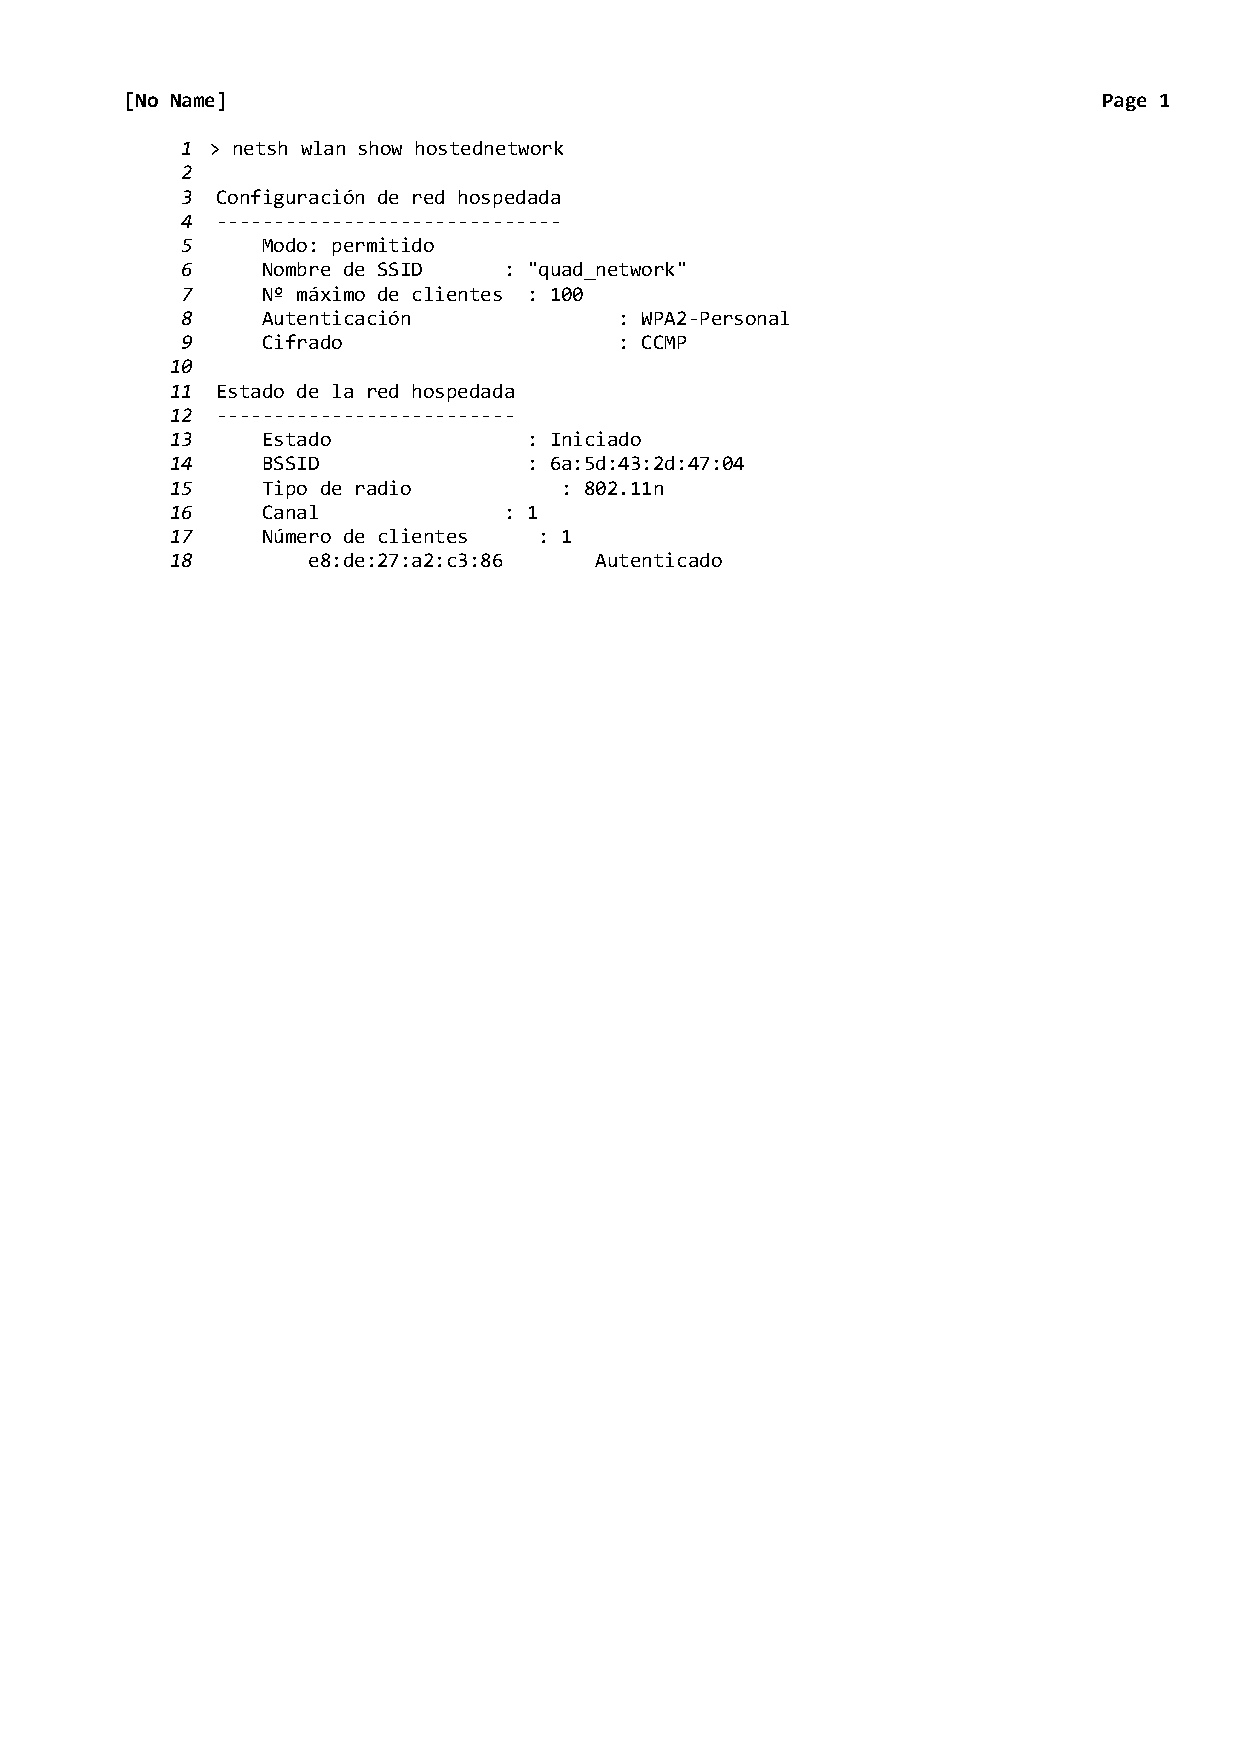
\includegraphics[width=0.95\textwidth,clip,trim={3.5cm 20cm 0 2.3cm}]{./files/shownetwork.pdf}

		In this case the Raspberry Pi's MAC address is \texttt{e8:de:27:a2:c3:86}, showing that the OCAS is connected to the GCS via the ad-hoc network

\end{enumerate}
